\section{\label{sec:resonances}Comparison of Data to Known Resonances}

In this section we show a series of figures depicting known resonances with the \abbr{g12} data. The reader is encouraged to compare the masses and widths measured with the PDG\cite{pdg}.

\begin{figure}[htpb]\begin{center}
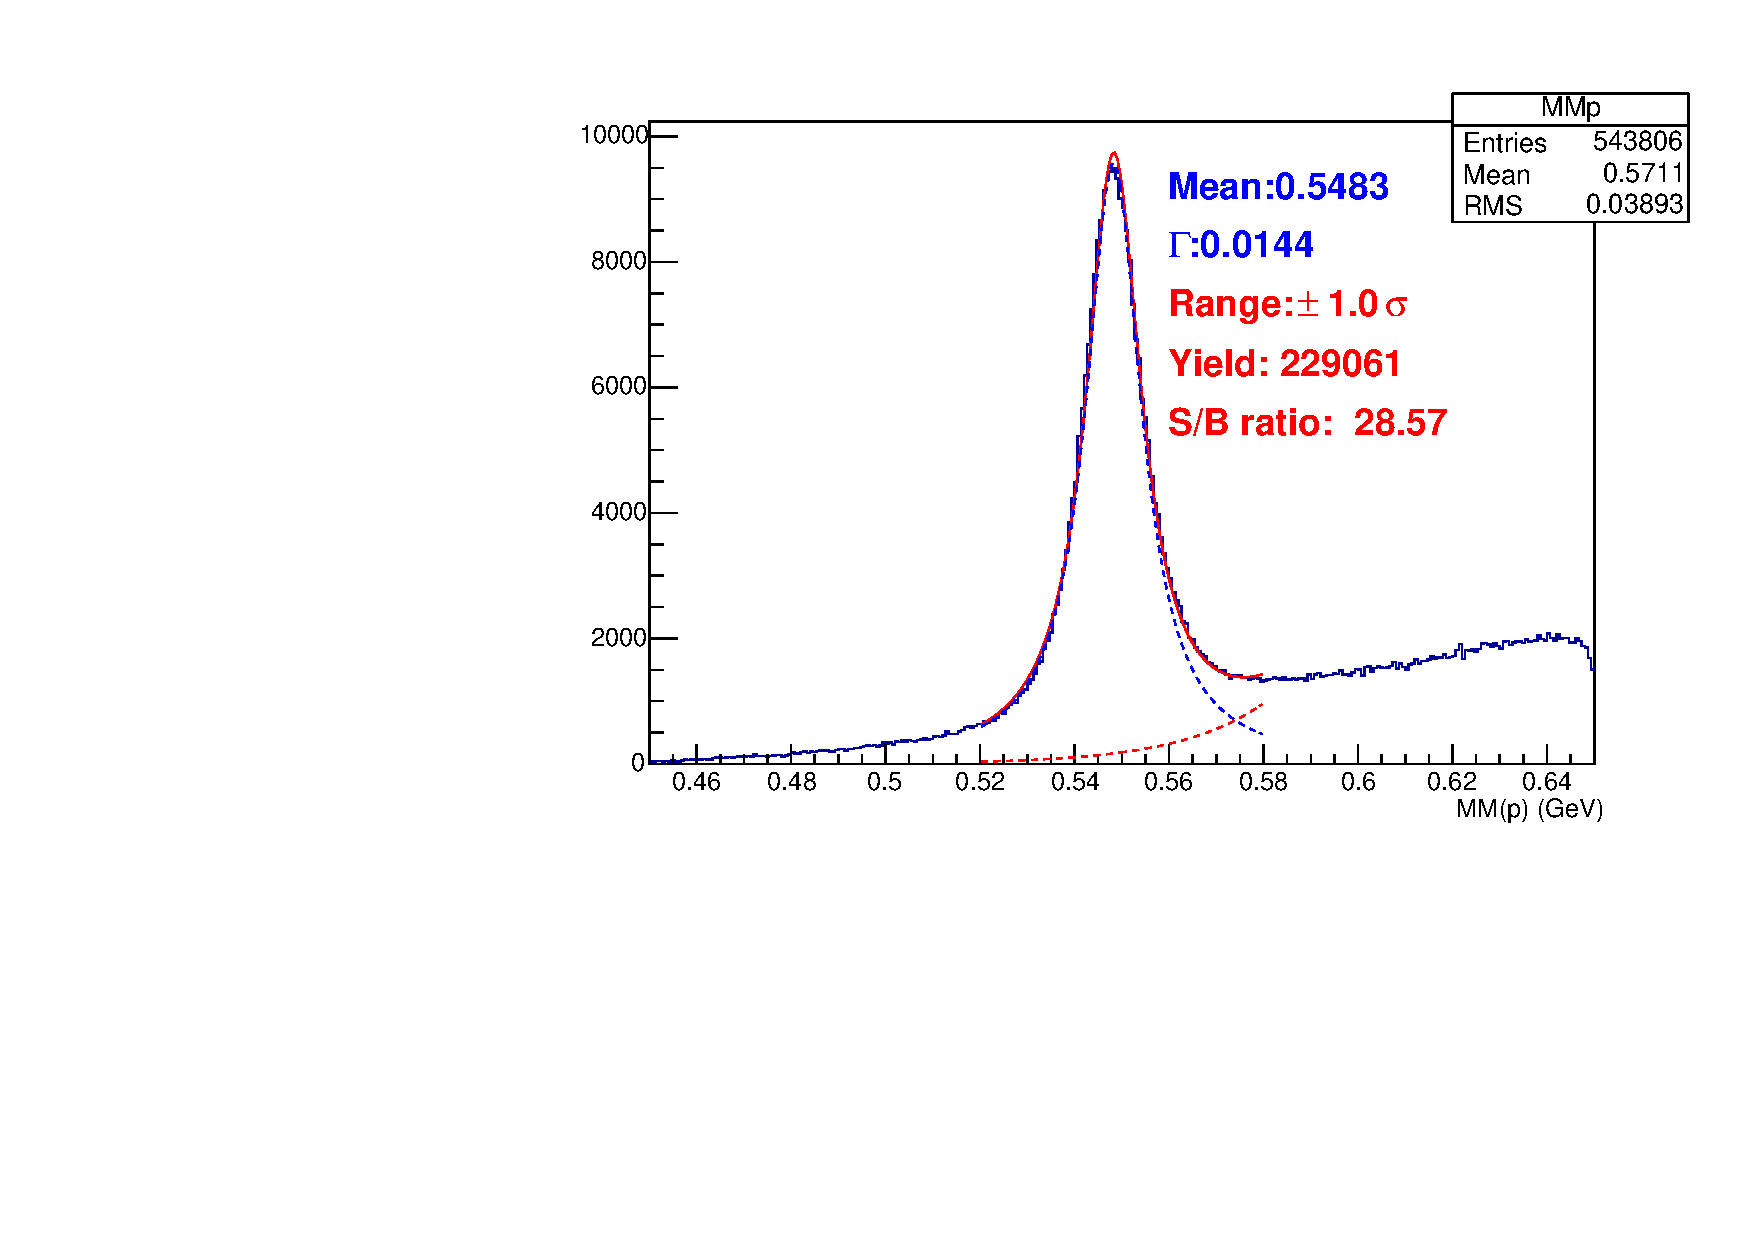
\includegraphics[width=0.4\columnwidth,angle=-90]{{figures/resonances/MMp-eta}.pdf}
\caption[]{\label{fig:resonances.eta}Missing mass off proton showing the η resonance with a measured mass of 548~MeV.}
\end{center}\end{figure}

\begin{figure}[htpb]\begin{center}
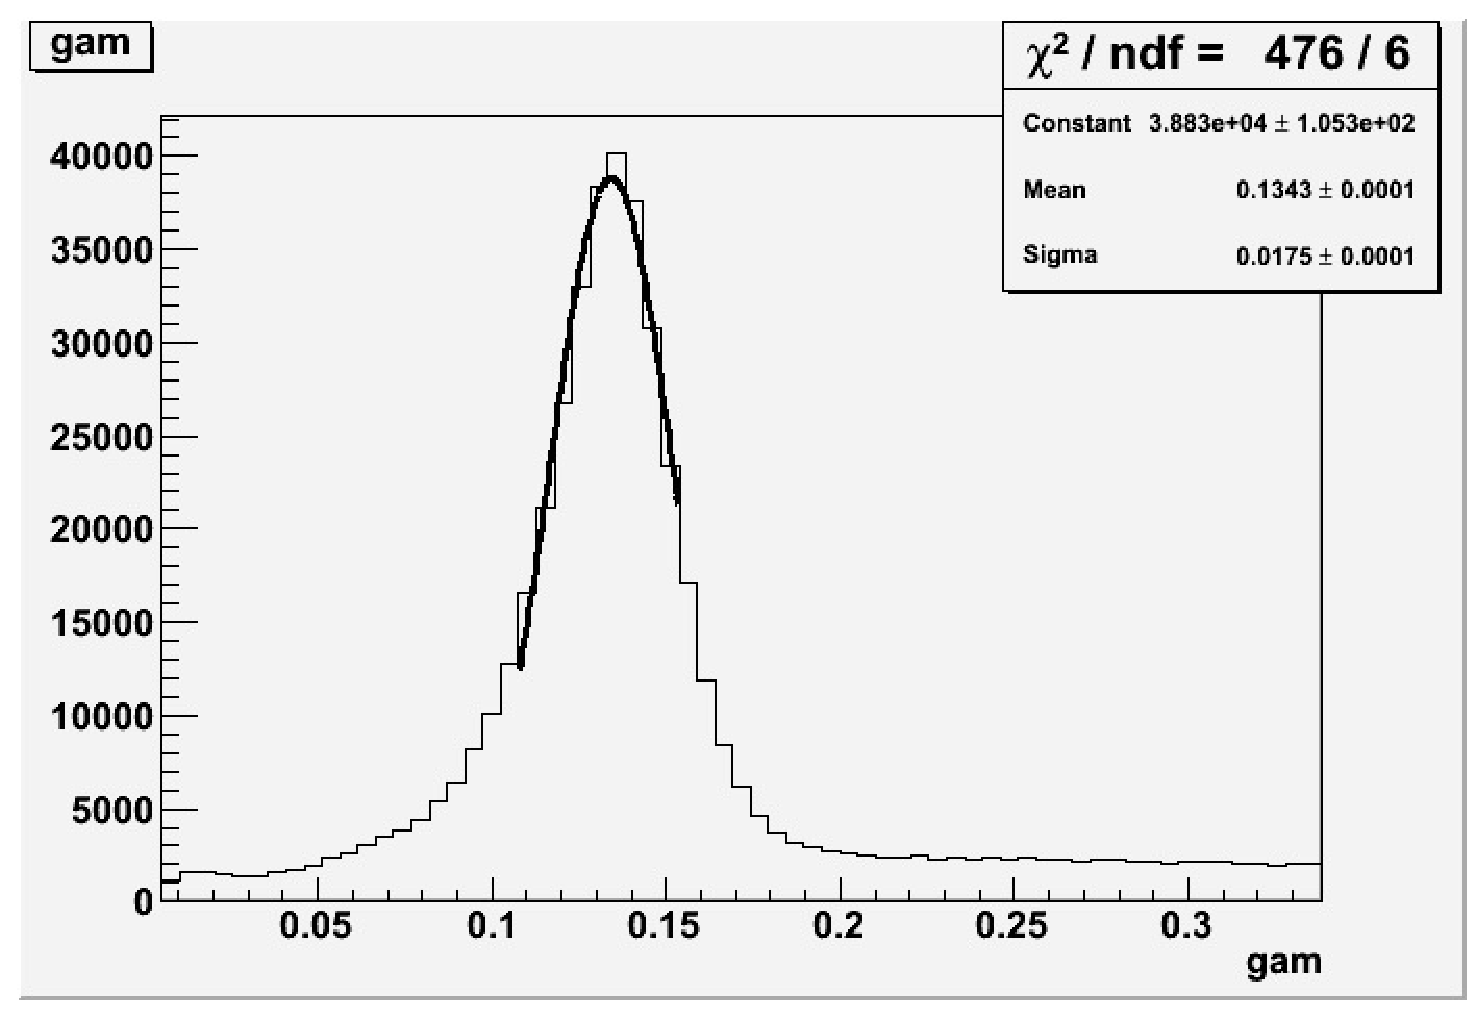
\includegraphics[width=0.4\columnwidth]{{figures/resonances/2gamma-pi0-p2pi2g}.eps}
\caption[]{\label{fig:resonances.2gamma.pi0}Invariant mass of two final-state photons showing the π$^0$ meson.}
\end{center}\end{figure}

\begin{figure}[htpb]\begin{center}
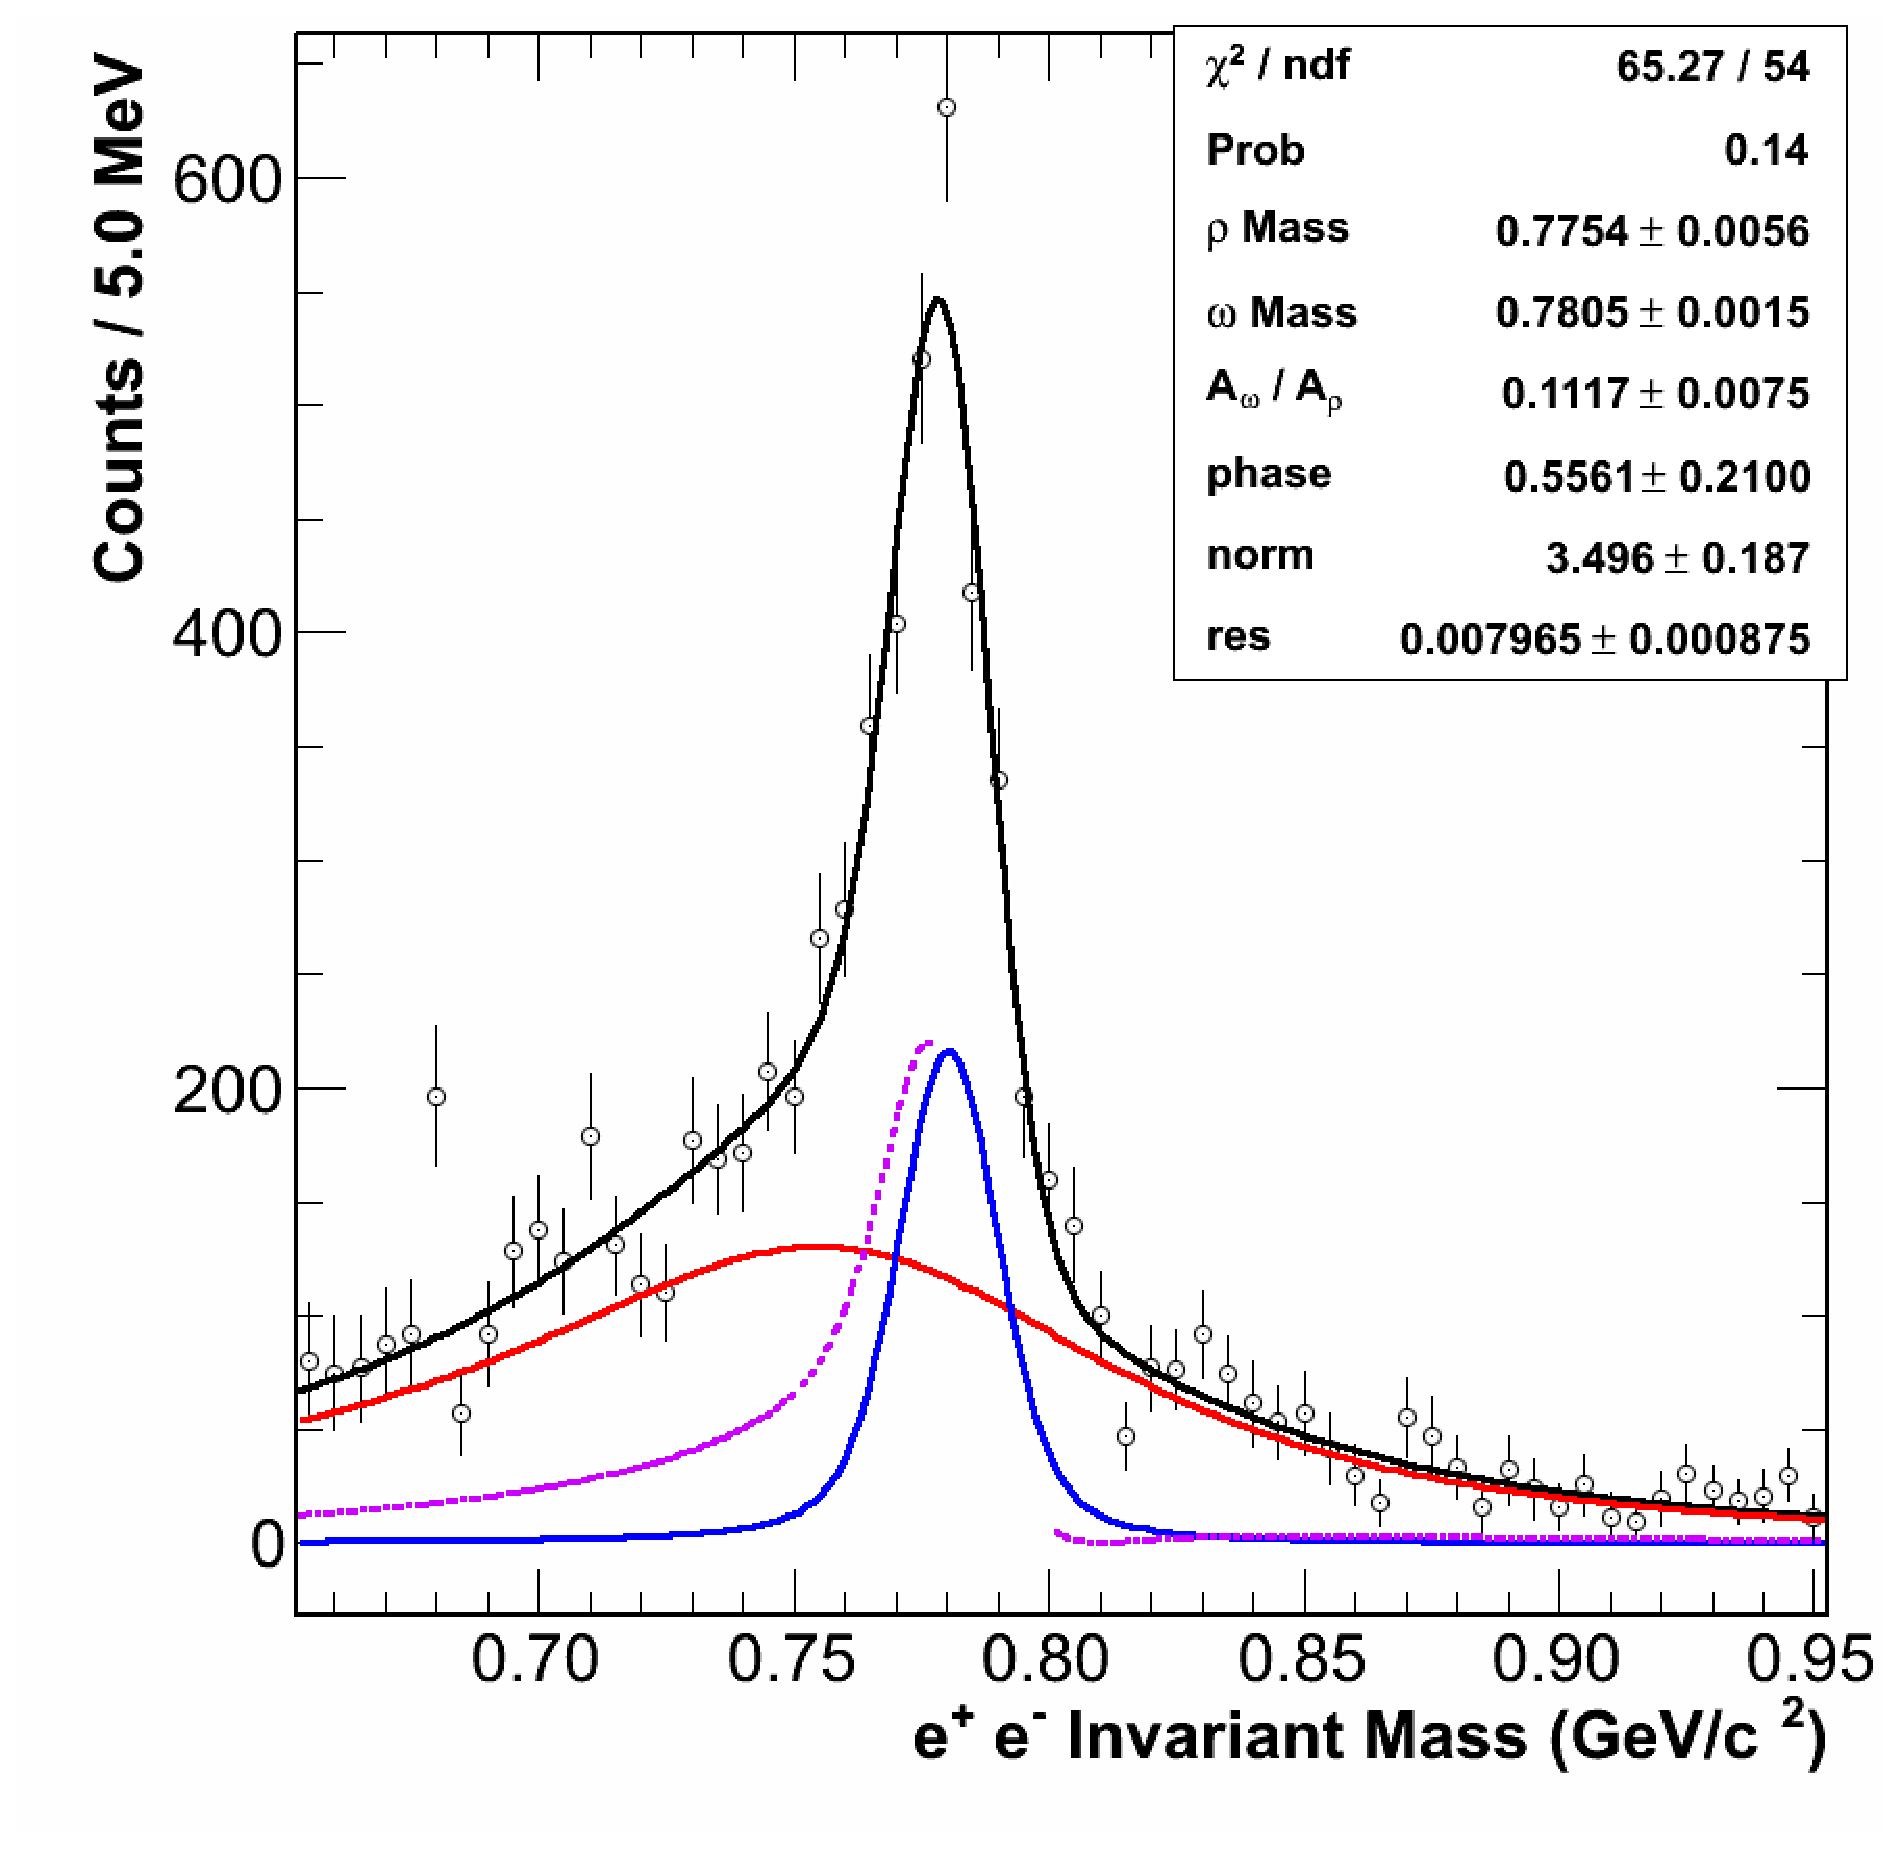
\includegraphics[width=0.4\columnwidth]{{figures/resonances/Sys_NormalRange}.eps}
\caption[]{\label{fig:resonances.ee.eho_omega}Invariant mass of electron and positron pair showing the (mixed) ρ and ω mesons.}
\end{center}\end{figure}

